\documentclass{beamer}
\usetheme{Boadilla}
\usecolortheme{spruce}

\usepackage[english,romanian,magyar]{babel}       
\usepackage[utf8]{inputenc}
\usepackage{graphicx}
\usepackage{caption}
\usepackage[absolute,overlay]{textpos}
\usepackage{subfig}
\usepackage{url}


\title[Artistic style transfer]{Párhuzamos képstílus átruházás konvolúciós neuronhálókkal}
\author[Szilágyi Ervin]{Szerző: Szilágyi Ervin\\{\small Témavezető: Dr. Iclănzan Dávid}}
\institute[Sapientia EMTE]{Sapientia Eredélyi Magyar Tudományegyetem \\ Műszaki és Humántudományok kar \\ Szoftverfejlesztés szak}
\date{\today}

\newcommand{\credit}[1]{\par\hfill \footnotesize \tiny Forrás:~\itshape#1}

\begin{document}
	\begin{frame}
		\titlepage
	\end{frame}

	\section{Bevezető}
	
	\begin{frame}
		\frametitle{Mi értünk stílusátruházás alatt?}
		\begin{center}
			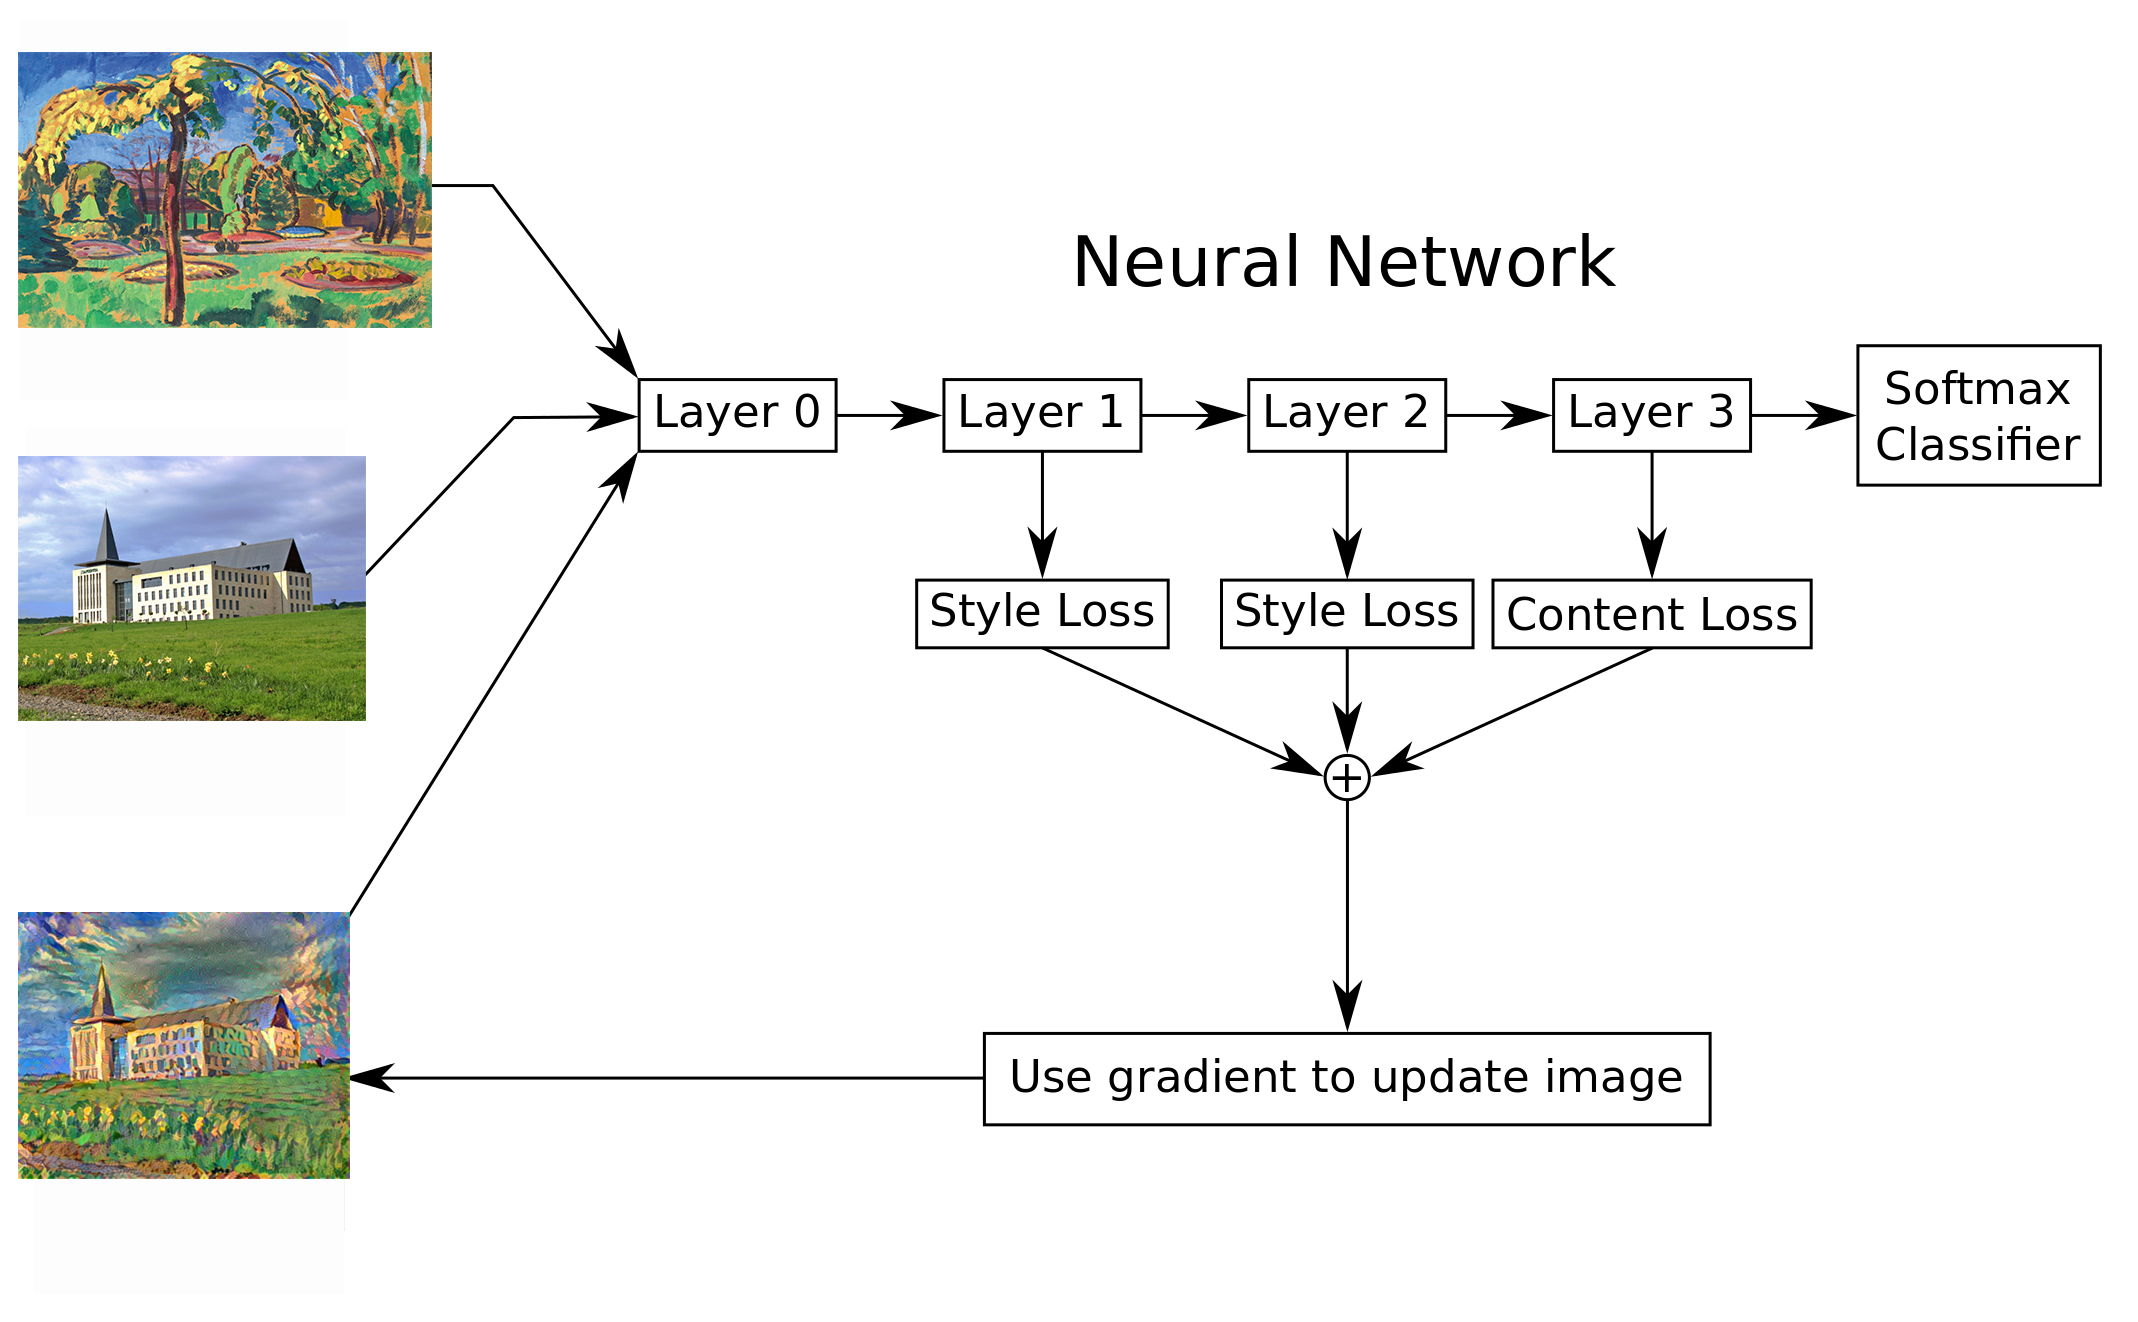
\includegraphics[scale=0.15]{system_presentation.png}
		\end{center}
	\end{frame}
	
	\begin{frame}
		\frametitle{A dolgozat célja}
		\begin{itemize}
			\item Grafikus felhasználói felülettel rendelkező alkalmazás fejlesztése 
			\item Gépi tanulást (deep learning) alkalmazó rendszer tervezése és megvalósítása
			\item Híres magyar festők ismertebb műveinek művészeti stílusát átruházni képekre / mozgóképekre
			\item Párhuzamos gépi tanítási folyamat ami kihasználja a GPU által biztosított párhuzamosítási lehetőségeket
		\end{itemize}
	\end{frame}

	\begin{frame}
		\frametitle{A Tensorflow könyvtár bemutatása}
		\begin{center}
			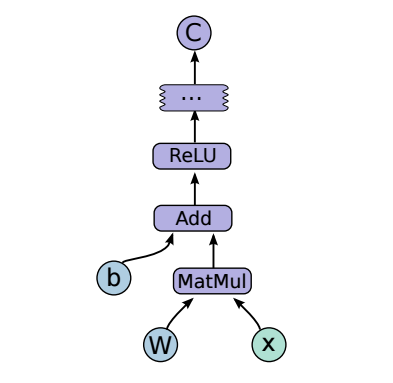
\includegraphics[scale=0.5]{tensorflow_graph.png}
			\captionof{figure}{Tensorflow számítási gráf}
			\credit{Google Research Team - TensorFlow: Large-Scale Machine Learning on Heterogeneous Distributed Systems}
			\label{tensorflow_graph}
		\end{center}
	\end{frame}

	\begin{frame}
		\frametitle{Párhuzamos tanítás a Tensorflow segítségével}
		\begin{figure}[!htbp]
			\centering
			\subfloat[Adatpárhuzamos megközelítés]{
				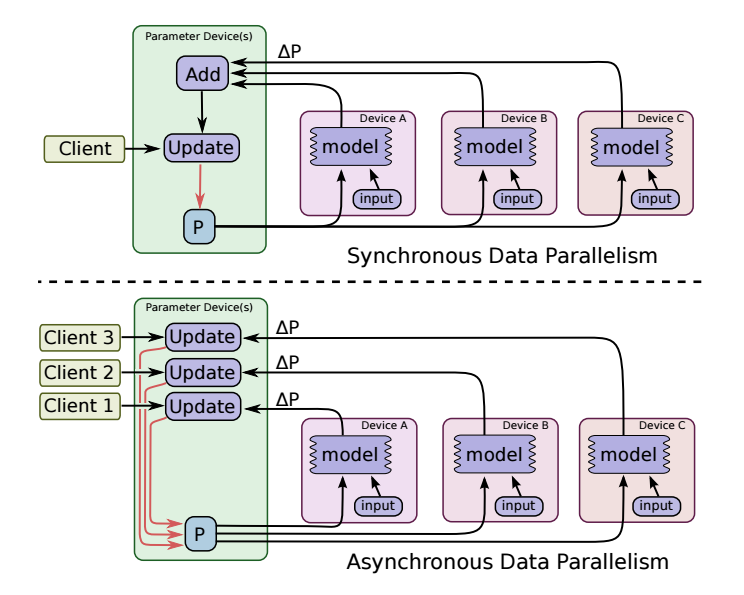
\includegraphics[width=60mm]{data_parallel_tf_model.png}
			}
			\subfloat[Feladatpárhuzamos megközelítés]{
				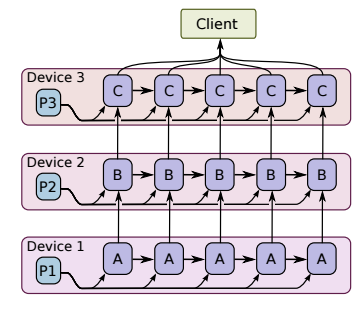
\includegraphics[width=40mm]{task_parallel_tf_model.png}
			}
			\caption{Párhuzamos tanítás}
			\credit{Google Research Team - TensorFlow: Large-Scale Machine Learning on Heterogeneous Distributed Systems}
		\end{figure}
	\end{frame}

	\section{Megvalósítás}
	\subsection{Statikus kép tanítása}
	
	\begin{frame}
		\frametitle{A rendszer tanítása}
		\begin{itemize}
			\item "Deep learning" tanítási metódus
			\item Előre betanított neuronháló (VGG19: 16 konvolúciós réteg, 5 pooling réteg)
			\item Statikus kép esetében külön tanításra kerül a bemeneti kép és a stílus kép is
			\item Mozgókép esetében minden képkocka tanításra kerül
			\item Temporális összefüggések a képkockák között
		\end{itemize}
	\end{frame}
	
	\begin{frame}
		\frametitle{A tanításhoz használt neuronháló}
		\begin{center}
			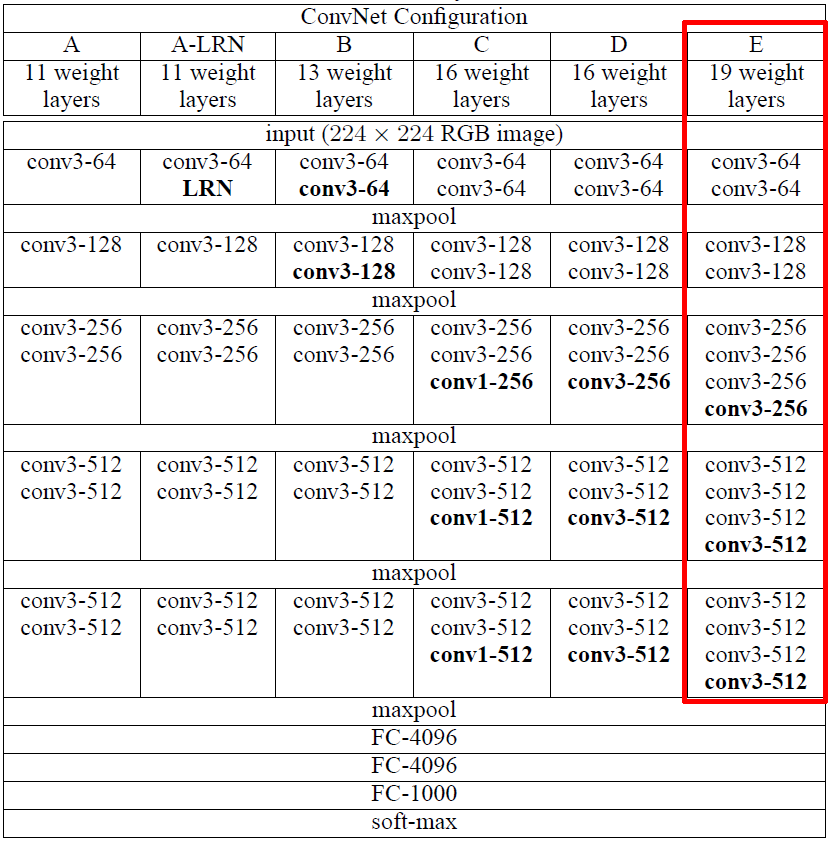
\includegraphics[scale=0.2]{VGG19.png}
			\captionof{figure}{VGG-19 háló szerkezete}
			\credit{Simonyan, K., Zisserman, A. - Very Deep Convolutional Networks for Large-Scale ImageRecognition}
		\end{center}
	\end{frame}

	\begin{frame}
		\frametitle{A bemeneti kép tanítása}
		\begin{itemize}
			\item A konvolúciós szűrök tartalmazzák a kép sajátosságait
			\item Egy adott betanított réteg válasza egy bemeneti képre vizualizálható, ha fehér zaj képre értékeljük ki azt
		\end{itemize}
			
		A bemeneti kép veszteségfüggvénye felírható mint:
		\begin{equation}
			L_{content}(\vec{x}, \vec{r}, l) = \frac{1}{2}\sum{R^l_{ij} - W^l_{ij}}
		\end{equation}
		
		Ahol:
		\begin{itemize}
			\item \(\vec{x}\) - a bemeneti képet
			\item \(R^l\) - az l-edik réteg válasza a bemeneti képre
			\item \(W^l\) - az l-edik réteg válasza a fehér zaj bemenetre
			\item \(\vec{r}\) - pedig azt a kimeneti képet jelenti amit a rendszer generál a rétegek tulajdonságaiból
		\end{itemize}
		
		Kiértékelt réteg: \(conv4\_2\)
	
	\end{frame}

	\begin{frame}
		\frametitle{A stílus kép tanítása}
		\framesubtitle{A Gramm-matrix ismertetése}
		
		\begin{itemize}
			\item A Gramm mátrix egy szorzatot jelen egy adott vektorhalmaz összes elemei között.
			\item Hogyha adott egy vektorhalmazunk \(v_1...v_n\), akkor a \(G\) Gramm mátrixot a következő eljárás szerint határozzuk meg:
				\begin{equation}
					G_{ij} = v_i \cdot v_j
				\end{equation}
			\item A Gramm mátrix \(ij\) pozíciójában elhelyezkedő elem megadja, hogy egy adott réteg \(i\)-dik tulajdonsága mennyire teljesül a \(j\)-dik tulajdonság jelenlétében,
		\end{itemize}
	\end{frame}

	\begin{frame}
		\frametitle{A stílus kép tanítása}
		\framesubtitle{A veszteségfüggvény meghatározása}
		
		Ha az \(l\) rétegnek \(N\) szűrője van, akkor felírható \(G \in R^{N_l*N_l}\) Gramm-mátrix, ahol:
		\begin{equation}
			G^l_{ij} = \sum_{k} F^l_{ik} \cdot F^l_{jk}
		\end{equation}
		
		A veszteségfüggvény egyetlen rétegre felírható mint a fehér zaj kép Gramm mátrixa és a stílus kép Gramm mátrixának átlagos négyzetes hibájaként:
		 
		\begin{equation}
			E_l = \frac{1}{4N^2_l M^2_l} \sum_{i,j} (G_{ij} - A_{lj})^2
		\end{equation}
		
		\begin{equation}
			L_{style}(\vec{a}, \vec{x}) = \sum w_lE_l
		\end{equation}
		
	\end{frame}

	\begin{frame}
		\frametitle{A stilizált kép tisztítása}
		\framesubtitle{Total Variation Denoising}
		
		A stilizált képet és eltoljuk X koordináta mentén egy pixellel, majd az Y koordináta mentén is eltoljuk egy pixellel.
		\begin{equation}
			L_{tv}(\vec{a}, \vec{x}) = \sum_{i,j} \left|(X_{ij} - A_{{i+1}j})\right| + \sum_{i, j} \left|(X_{ij} - A_{i {j+1}})\right|
		\end{equation}
	\end{frame}

	\begin{frame}
		\frametitle{Tanítási függvény}
		
		\begin{equation}
			L = L_{content} + L_{style} + L_{tv}
		\end{equation}
		
		Optimalizációs algoritmus: ADAM ( Adaptive Moment Estimation). felhasználja a elsődleges, valamint a másodlagos gradiensek átlagát ahhoz, hogy a veszteségfüggvényt minimalizálja.
		
	\end{frame}

	\subsection{Mozgókép tanítása}
	
	\begin{frame}
		\frametitle{Mozgókép tanítása}
		\framesubtitle{Naív megközelítés}
		A videót feldaraboljuk képkockákra, majd az összes képkockára átruházzuk a stílust.
		\newline
		
		Előnyei:
		\begin{itemize}
			\item Gyors.
		\end{itemize}
		
		Hátrányai:
		\begin{itemize}
			\item Nincs folyamatos átmenet a képkockák között
			\item Artifacts, pop-ins
		\end{itemize}
	\end{frame}

	\begin{frame}
		\frametitle{Mozgókép tanítása}
		\framesubtitle{Optical flow bevezetése}
		\begin{center}
			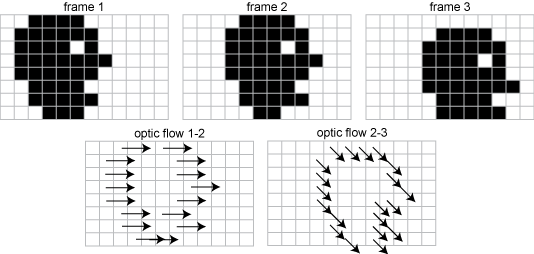
\includegraphics[scale=0.6]{optical_flow.png}
			\credit{\url{http://www.scholarpedia.org/article/Optic_flow}}
			\captionof{figure}{Optical flow szemléltetése}
		\end{center}
	\end{frame}

	\begin{frame}
		\frametitle{Mozgókép tanítása}
		\framesubtitle{A háló inicializálása}
		A cél:
		\begin{itemize}
			\item A mintázatok ugyanabba a pontba konvergáljanak
			\item "Flickering" jelenség elkerülése
		\end{itemize}
	
		Megoldás - a neuronhálót a következőképpnek inicializáljuk:
		\begin{itemize}
			\item Optical flow-t számolunk az elöző stilizált képkocka és a mostani képkocka között
			\item Az elöző stilizált képkockát trozítjuk az optical flow vektorai szerint
		\end{itemize}
	\end{frame}

	\begin{frame}
		\frametitle{Mozgókép tanítása}
		\framesubtitle{Temporális összeföggések a képkockák között}
		
		Jelölje \(w(u, u)\) az előre történő optical flow-t, valamint \(\hat{w}(\hat{u}, \hat{u})\) a visszafele történő optical flow-t. Az előre történő optical flow torzítása:
		\begin{equation}
			\tilde{w}(i, j) = w((i, j) + \hat{w}(i, j))
		\end{equation}
		
		A mozgás néküli és újonnan megjelenő objektumok nélküli zónák azok amelyekre a következő egyenlőtlenség fenn áll:
		\begin{equation} \label{eq:1}
			|\tilde{w} + \hat{w}|^2 > 0.01(|\tilde{w}|^2 + |\hat{w}|^2) + 0.5
		\end{equation}
		
		A mozgási határok pedig meghatározhatóak:
		\begin{equation} \label{eq:2}
			|\nabla\hat{u}| + |\nabla\hat{v}| > 0.01|\tilde{w}|^2 + 0.002
		\end{equation}
		
		\begin{figure}[!htbp]
			\centering
			\subfloat[Frame00001]{
				
\includegraphics[width=30mm]{input_frame00001.jpg}
			}
			\subfloat[Frame00002]{
				
\includegraphics[width=30mm]{input_frame00002.jpg}
			}
			\hspace{0mm}
			\subfloat[Forward consistency matrix]{
				
\includegraphics[width=25mm]{forward.jpg}
			}
			\label{consistency_weights}
		\end{figure}
		
	\end{frame}

	\begin{frame}
		\frametitle{Mozgókép tanítása}
		\framesubtitle{Veszteségfüggvény meghatározása}
		
		\begin{equation} \label{eq:2}
			L_{temporal}(x, w, c) = \frac{1}{D}\sum_{k=1}^{D}c_k\cdot(x_k-w_k)^2
		\end{equation}
		Ahol: \\ 
		C - mátrix: mozgási határokra 1-est rakunk, a többi érték 0-ás \\
		x - bemeneti kép \\
		W - előző torzított kép \\
		\vspace{1cm}
		Végső tanítási függvény:
		\begin{equation}
			L = L_{content} + L_{style} + L_{tv} + L_{temporal}
		\end{equation}
		
	\end{frame}

	\subsection{A szoftvet architektúrája}
	
	\begin{frame}
		\frametitle{A szoftvet architektúrája}
		\framesubtitle{A szoftver komponensei}
		\begin{center}
			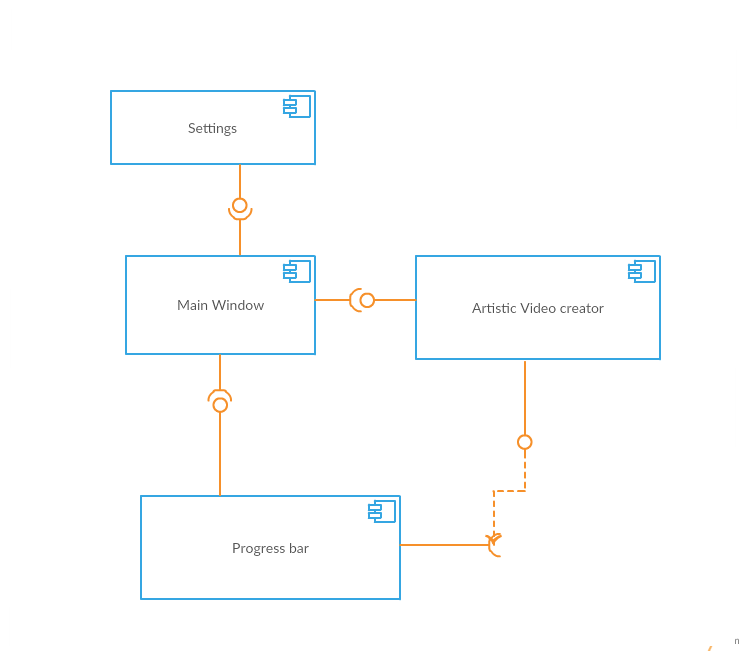
\includegraphics[scale=0.3]{component_diagram.png}
		\end{center}
	\end{frame}

	\begin{frame}
		\frametitle{A szoftvet architektúrája}
		\framesubtitle{Többszálas megvalósítás}
		\begin{center}
			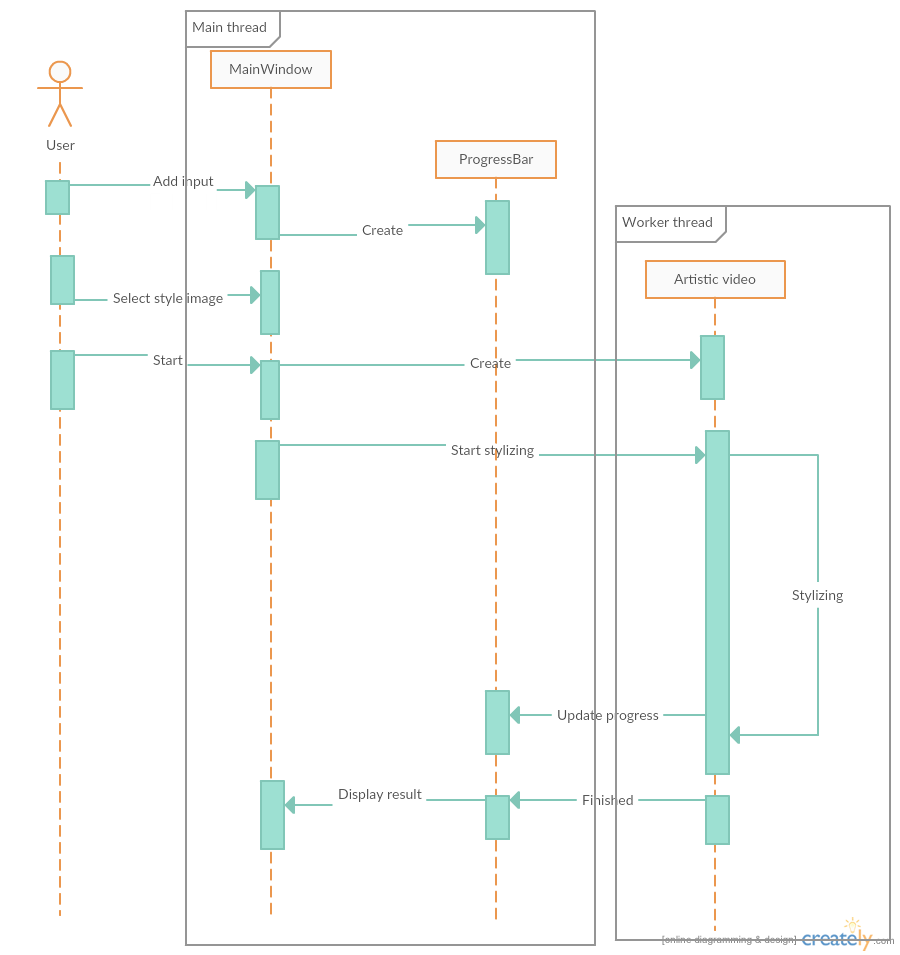
\includegraphics[scale=0.2]{seq_diagram.png}
		\end{center}
	\end{frame}

	\begin{frame}
		\frametitle{A felhasználói felület}
		\begin{itemize}
			\item Python
			\item PyQt5
		\end{itemize}
		\begin{center}
			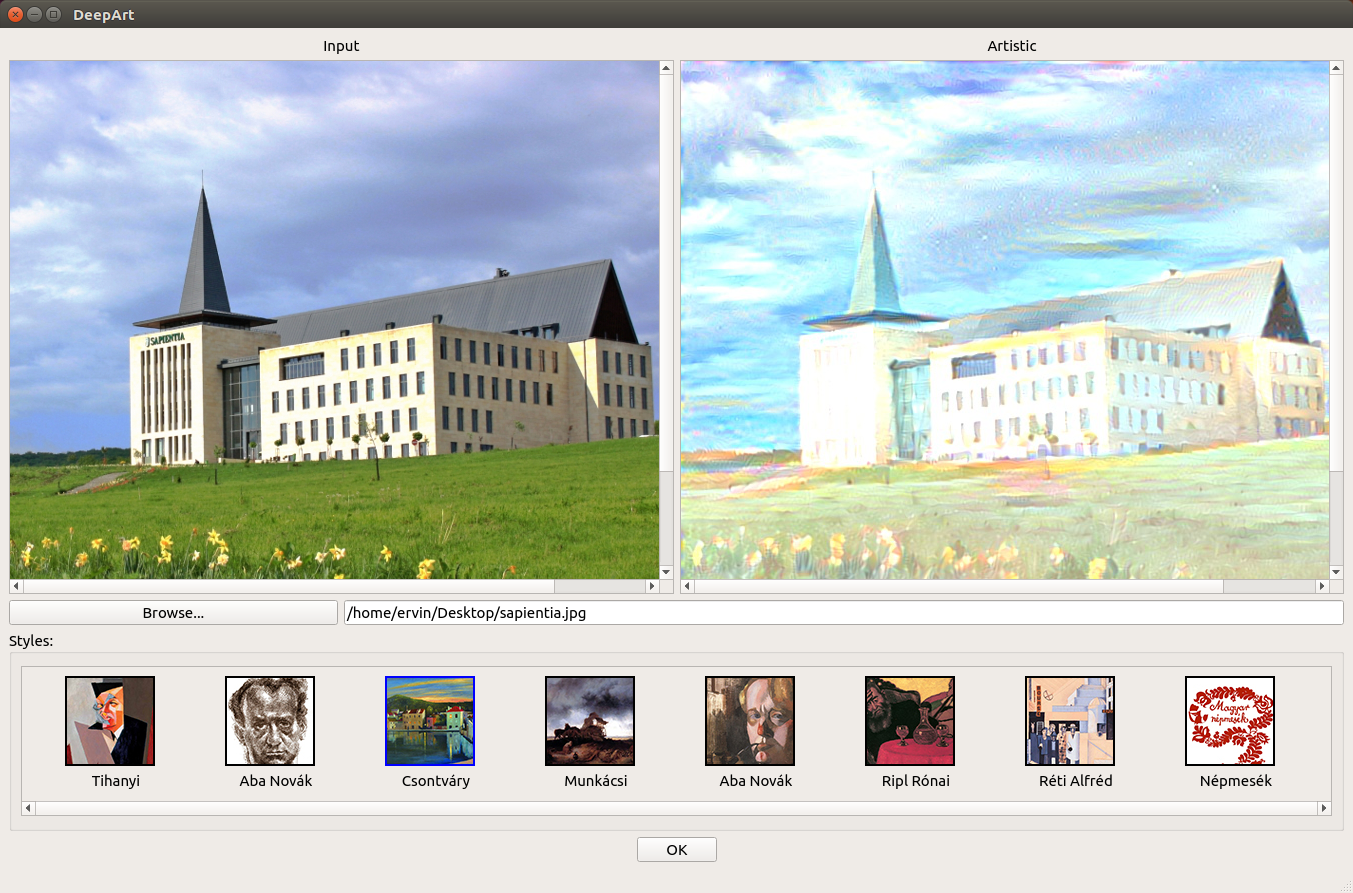
\includegraphics[scale=0.18]{main_ui.png}
		\end{center}
	\end{frame}

	\begin{frame}
		\frametitle{Stílusképek}
		\begin{figure}[!htbp]
			\centering
			\subfloat[\tiny{Aba Novak Vilmos - Önarckép}]{
				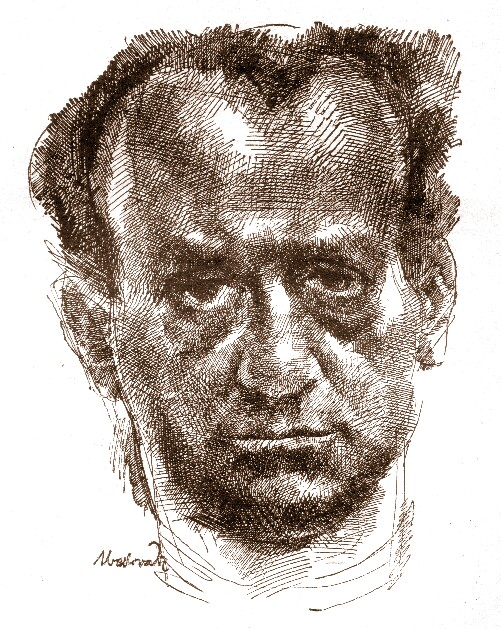
\includegraphics[width=20mm]{stylistic/styles/aba_novak_vilmos_onarckep.jpg}
			}
			\subfloat[\tiny{Aba Novak Vilmos - Selfportrait}]{
				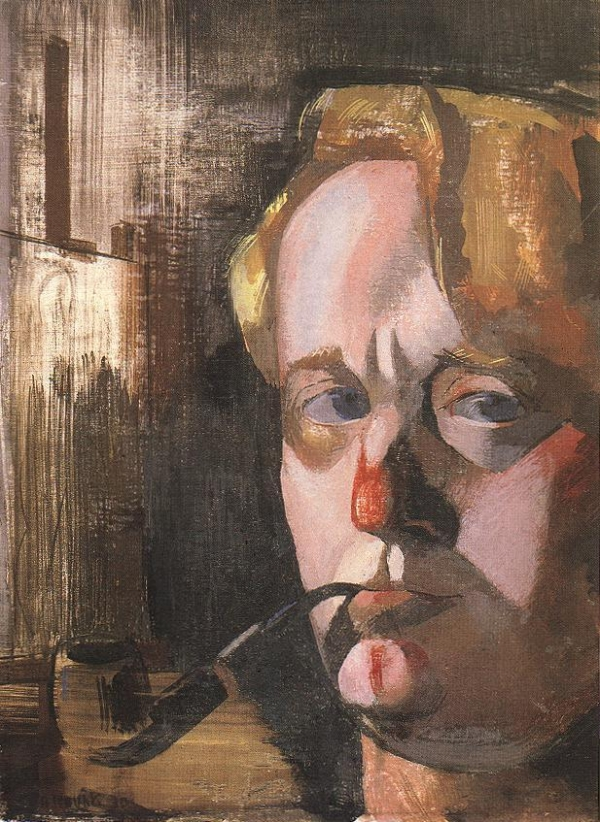
\includegraphics[width=20mm]{stylistic/styles/aba-novak_vilmos_selfportrait.jpg}
			}
			\subfloat[\tiny{Kosztka Tivadar} - Traui tájkép naplemente idején]{
				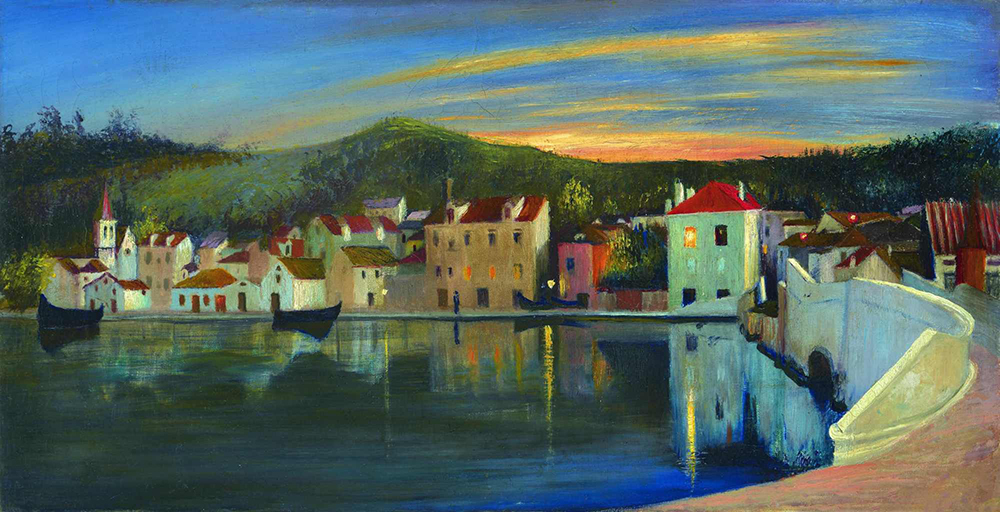
\includegraphics[width=20mm]{stylistic/styles/csontvary_kosztka_tivadar_traui_tajkep_naplemente_idejen.jpg}
			}
			\subfloat[\tiny{Grunwald Béla} - Parkrészlet Kecskeméten]{
				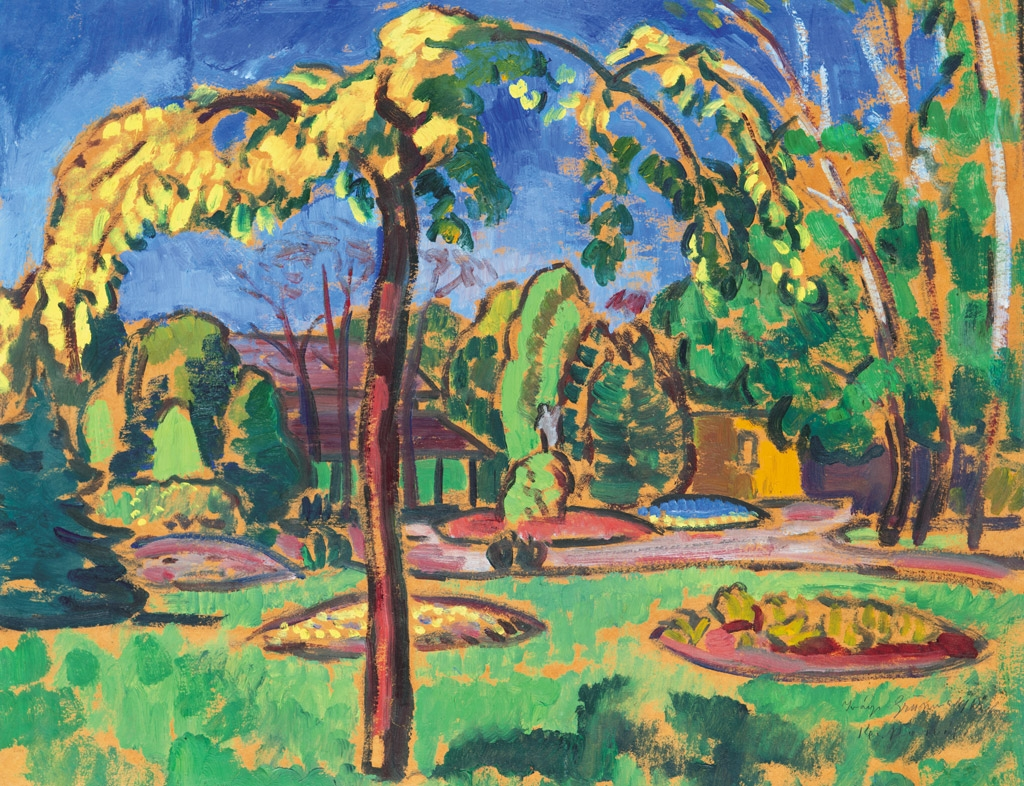
\includegraphics[width=20mm]{stylistic/styles/ivanyi_grunwald_bela_parkreszlet_kecskemeten.jpg}
			}
			\subfloat[\tiny{Munkácsi Mihály - Vihar a pusztán}]{
				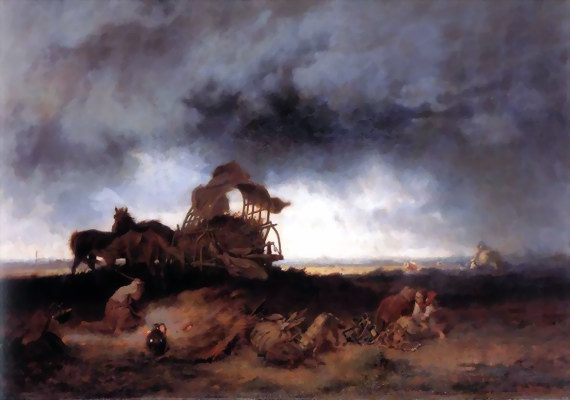
\includegraphics[width=20mm]{stylistic/styles/munkacsi_mihaly_vihar_a_pusztan}
			}
			\vspace{0cm}
			\subfloat[\tiny{Réti Alfréd}]{
				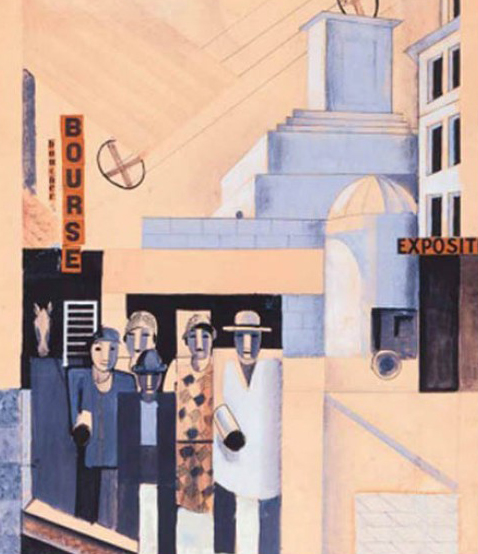
\includegraphics[width=20mm]{stylistic/styles/reti_alfred.jpg}
			}
			\subfloat[\tiny{Ripl-Rónai József - Apám és Piacsek...}]{
				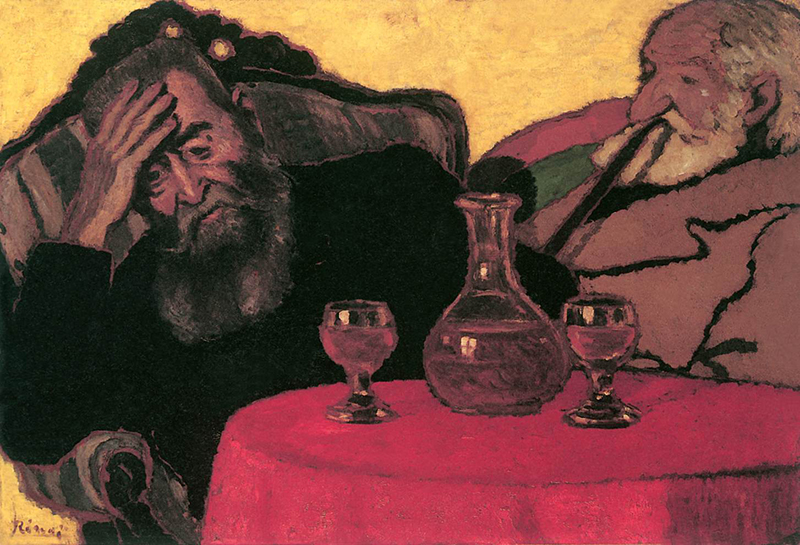
\includegraphics[width=20mm]{stylistic/styles/ripl_ronai_jozsef_apam_es_piacsek_bacsi_vorosbor_mellett.jpg}
			}
			\subfloat[\tiny{Tihanyi - Tzara}]{
				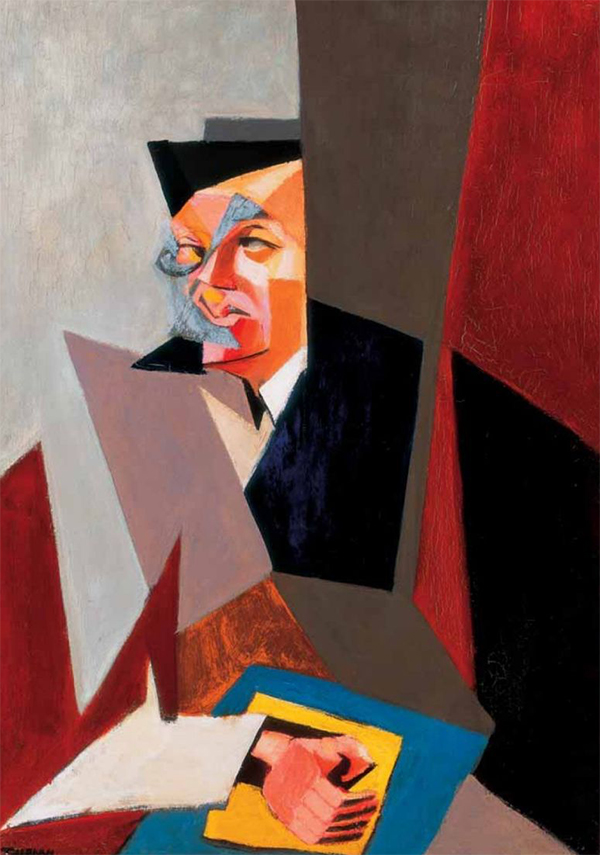
\includegraphics[width=20mm]{stylistic/styles/tihanyi_tzara.jpg}
			}
			\subfloat[\tiny{Magyar Népmesék}]{
				
\includegraphics[width=20mm]{stylistic/styles/magyar_nepmesek.jpg}
			}
			\caption{Stílusképek}
			\label{styles}
		\end{figure}
	\end{frame}

	\section{A rendszer tesztelése}
	
	\begin{frame}
		\frametitle{Mérések}
		\framesubtitle{A tesztkonfiguráció meghatározása}
		
		\begin{itemize}
			\item \textbf{Alaplap:} MSI Z170A-G45 GAMING
			\item \textbf{Processzor:} Intel(R) Core(TM) Skylake i7-6700 ("non-K") CPU @ 3.40GHz (Turbo Boost: 3.90GHz)
			\item \textbf{Videokártya:} GIGABYTE GeForce GTX 1080 G1 GAMING 8GB DDR5X 256-bit
			\item \textbf{RAM Memória:} Corsair Vengeance LPX Black 32GB DDR4 3000MHz
			\item \textbf{Merev lemez}: HyperX Savage SSD, 240GB, 2.5", SATA III
			\item \textbf{Operációs rendszer:} Ubuntu 17.04 LTS
		\end{itemize}
	\end{frame}

	\begin{frame}
		\frametitle{Egy képkockára történő stílusátruházási idő}
		
		\begin{columns}
			\column{0.5\textwidth}
			\begin{tabular}{ | l | l |}
				\hline
				Felbontás(pixel) & Idő(másodperc) \\ \hline
				$320 \times $240 & 23.126104 \\ \hline
				$640 \times $480 & 82.640347 \\ \hline
				$720 \times $480 & 93.487573 \\ \hline
				$800 \times $600 & 127.973041 \\ \hline
				$1024 \times $764 & 203.892024 \\ \hline
				$1280 \times $720 & 245.769916 \\ \hline
				$1366 \times $768 & 279.945757 \\ \hline
			\end{tabular}
			\column{0.5\textwidth}
			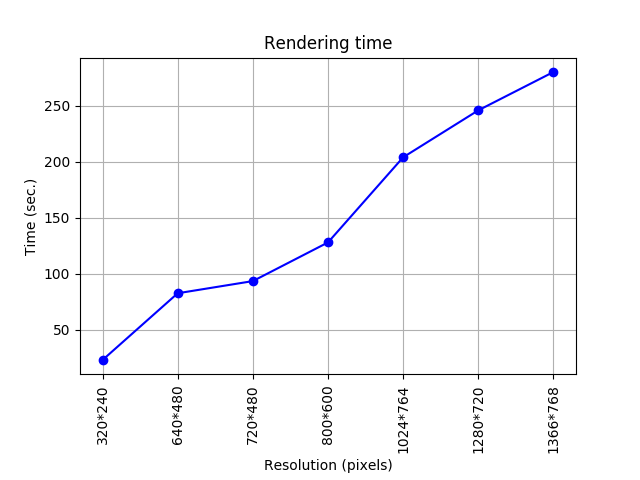
\includegraphics[scale=0.4]{time_per_res.png}
		\end{columns}
	\end{frame}

	\begin{frame}
		\frametitle{Videókártya memóriahasználata és kihasználtsága}
		
		\begin{columns}
			\column{0.5\textwidth}
			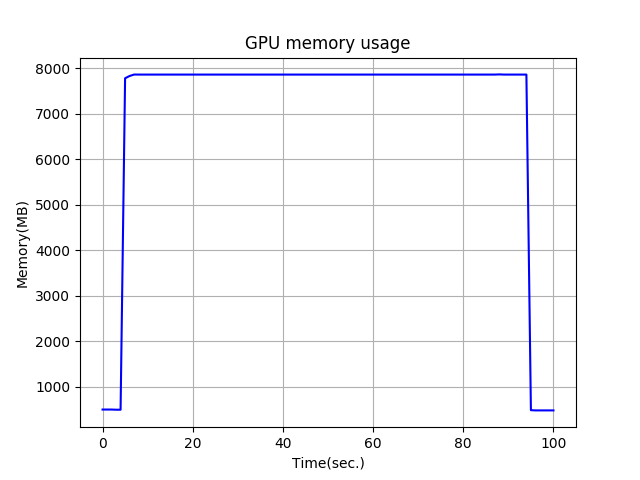
\includegraphics[scale=0.4]{gpu_memory_usage.png}
			\captionof{figure}{Memóriahasználat}
			\column{0.5\textwidth}
			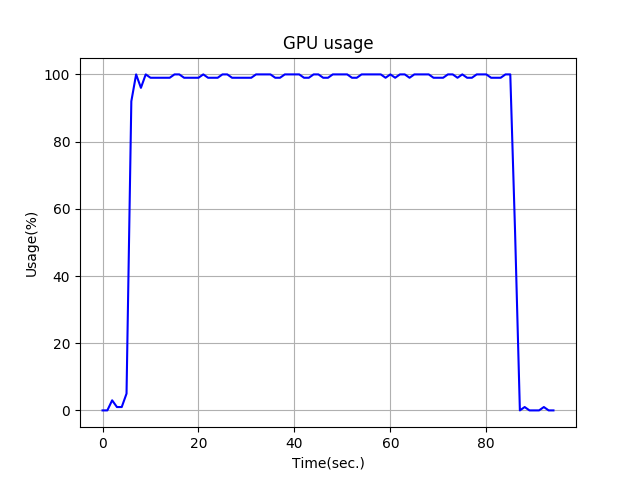
\includegraphics[scale=0.4]{gpu_usage.png}
			\captionof{figure}{Kihasználtság}
		\end{columns}
	\end{frame}

	\begin{frame}
		\frametitle{CPU - GPU összehasonlítás}
		\begin{center}
			\begin{tabular}{ | l | l | l | l| }
				\hline
				Felbontás(pixel) & GPU Idő(sec.) &  CPU Idő(sec.) & Gyorsulás\\ \hline
				$320 \times $240 & 23.126104 & 862.980290 & 37.316285\\ \hline
				$640 \times $480 & 82.640347 & 3487.931886 & 42.206162\\ \hline
				$800 \times $600 & 127.973041 & 5446.849902 & 42.562479\\ \hline
				$1024 \times $768 & 203.892024 & 8935.804122 & 43.826158\\ \hline
			\end{tabular}
			\begin{columns}
				\column{0.5\textwidth}
				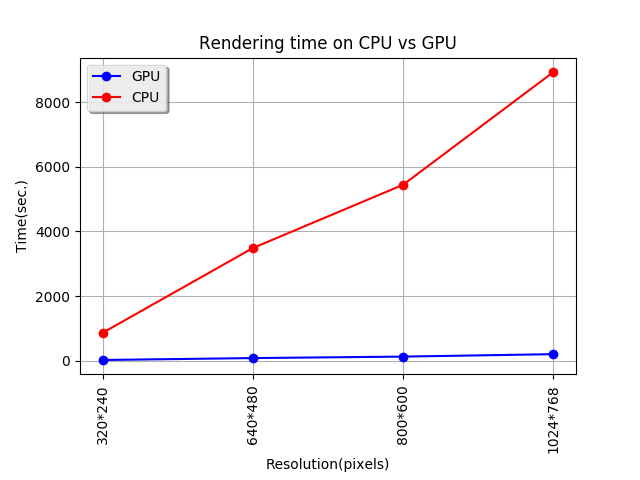
\includegraphics[scale=0.38]{cpu_vs_gpu.png}
				\column{0.5\textwidth}
				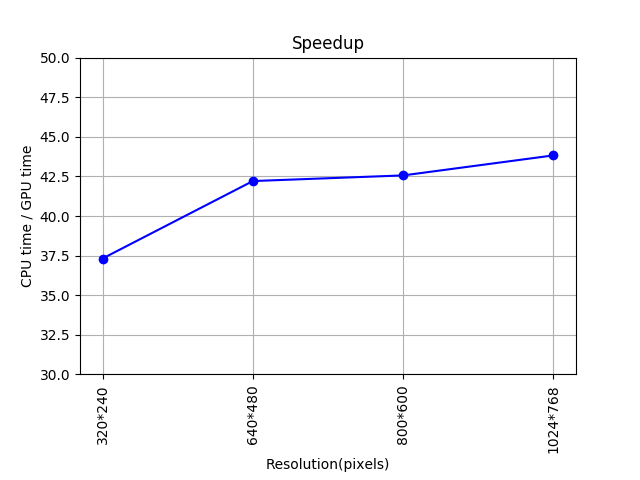
\includegraphics[scale=0.38]{speedup.png}
			\end{columns}
		\end{center}
	\end{frame}

	\begin{frame}
		\frametitle{Az Optical flow időigénye}
		\begin{center}
			\begin{columns}
				\column{0.5\textwidth}
				\begin{tabular}{ | l | l |}
					\hline
					Felbontás(pixel) & Idő(másodperc) \\ \hline
					$320 \times $240 & 3.700949 \\ \hline
					$640 \times $480 & 71.693549 \\ \hline
					$720 \times $480 & 75.388477 \\ \hline
					$800 \times $600 & 186.4160516 \\ \hline
					$1024 \times $764 & 371.140060 \\ \hline
					$1280 \times $720 & 466.996901 \\ \hline
					$1366 \times $768 & 481.25628 \\ \hline
				\end{tabular}
				\column{0.5\textwidth}
				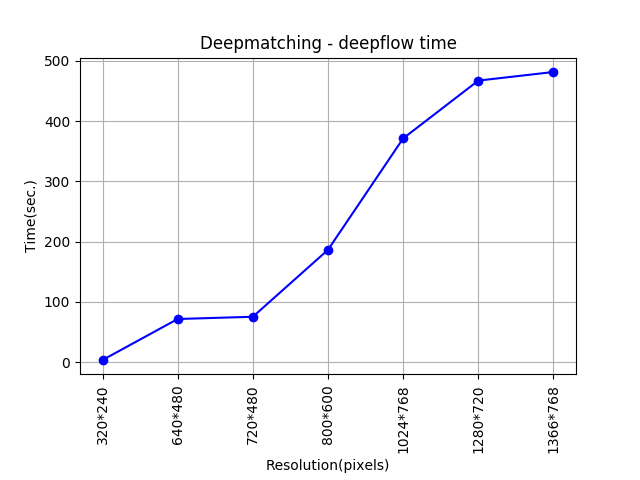
\includegraphics[scale=0.42]{deepmatching_deeplfow.png}
			\end{columns}
		\end{center}
	\end{frame}

	\begin{frame}
		\frametitle{Egy perces videóra történő stílusátvitel}
		24 FPS, 60 másodperc, 1440 képkocka
		\begin{center}
			\begin{columns}
				\column{0.5\textwidth}
				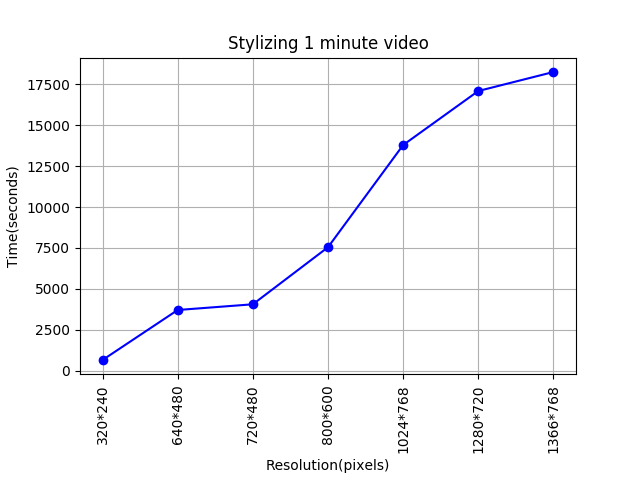
\includegraphics[scale=0.42]{one_min_video_opt_flow.png}
				\captionof{figure}{Optical flow használatával}
				\column{0.5\textwidth}
				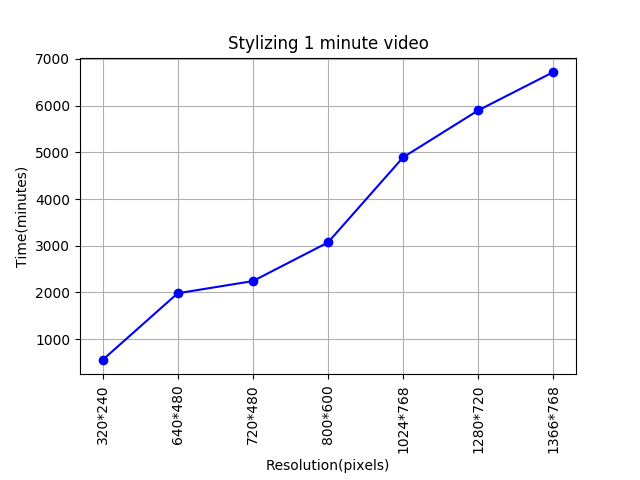
\includegraphics[scale=0.42]{one_min_video.png}
				\captionof{figure}{Optical flow használata nélkül}
			\end{columns}
		\end{center}
	\end{frame}
	
	\section{Összefoglaló}
	
	\begin{frame}
		\frametitle{Összefoglaló}
		\begin{itemize}
			\item Grafikus felhasználói felülettel rendelkező szoftver fejlesztése
			\item Magyar festők híres műveinek stíluást alkalmazni mindennapi képekre/mozgóképekre
			\item Képkockák közötti temporális összefüggések kihasználása mozgóképek esetében
			\item Tesztek, mérések elvégzése
		\end{itemize}
		
		\vspace{0.5cm}
		Továbbfejlesztési lehetőségek:
		\begin{itemize}
			\item Saját háló betanítása, más tanítási eljárás használata
			\item Optical flow algoritmus gyorsítása (párhuzamosítás, más algoritmusok kipróbálása)
			\item Teljes Windows-os támogatás
			\item Grafikus felület úrjatervezése, szépítése
			\item Cloud alapú szolgáltatás készítése
		\end{itemize}
		\vspace{0.5cm}
		\begin{center}
			Köszönöm a figyelmet!
		\end{center}
	\end{frame}
	
	
\end{document}